\chapter{Approach}
\section{System-model}\label{sec:model}
In this section, we define the system model that serves as the foundation for the concept of the generated task-sets.

\subsection{Task Model}\label{sec:task_model}
Part of the system model is a harmonic set of periodic tasks $\Tau=\{\Tau_i: i = 1, 2, \ldots, n\}$.
Due to being a harmonic task-set and its properties (see \cref{sec:scheduling}) the \textit{planning cycle}\cite{dar-tzenpengAssignmentSchedulingCommunicating1997} of $\Tau$ is defined by the \textit{\ac{LCM}} of all tasks' periods $\{P_1, \ldots, P_n\}$, resulting in the period $P_{max}$ of the task with the highest period.
Each task $\Tau_i$ is characterized by its period $P_i$, its list of possible execution times $\{CP_{i_1}, CP_{i_2}, \ldots\}$, and the set of related jobs $\tau_i=\{\tau_{i_0}, \tau_{i_1}, \dots, \tau_{i_m}; m = \frac{P_{max}}{P_i} - 1\}$.

Each job $\tau_{i_j}$ is described by the release time $r_{i_m}$, the begin of the next period $P_i+1$ is equal to the implicit deadline $d_i$, the jobs computational time $C_{i_m}$.
The release time $r_{i_m}$ per job is set to be aligned with the period beginning with $0$.
\begin{center}
	$r_{i_m} = P_i \times m$ \\
	$d_{i_m} = P_i + r_{i_m}$
\end{center}
\todo{explain chains and their length}

\subsection{Hardware Model}\label{sec:hardware_model}
The generated model is designed to be a meta model with no constraints on hardware specifications, making it hardware independent.
No further details about the hardware are provided.

\subsection{Execution Model}\label{sec:execution_model}
In the execution model, a preemptive scheduler using \ac{RMS} (see \cref{sec:scheduling}) is employed to manage the periodic tasks. 
The scheduler operates by assigning each task $\Tau_i$ a priority inversely proportional to its period $P_i$ \ref{liuSchedulingAlgorithmsMultiprogramming1973}.
Tasks with shorter periods receive higher priorities and are scheduled more frequently.
Higher-priority tasks can preempt lower-priority tasks.
If a higher-priority task becomes ready to execute while a lower-priority task is running, the scheduler will interrupt the lower-priority task and allocate the processor to the higher-priority task.
The generated schedule is represented by a list of time frames associated to a job being run in that time frame $sched = \{begin, end, \tau_{i_j}\}$.

Making use of the \ac{RMS} in combination with the in \cref{sec:task_model} mentioned harmonic task-set it is possible to reach utilizations up to $1$ \cite{liuSchedulingAlgorithmsMultiprogramming1973}.


\cite{dar-tzenpengAssignmentSchedulingCommunicating1997}


\section{Concept}
\label{sec:concept}
The general workflow involves several key steps. 
\begin{enumerate}
	\item Generate period times based on the server model.
	\item Create task chains and identify any missing links within these chains.
	\item Distribute the load across each period and generate tasks with lower execution times to balance the workload.
	\item Connect tasks and create conditions, considering the idea of workloads with resources attached, such as inter-task communication.
	\item Spread the server model into multiple server instances.
	\item Build a scheduler and perform a schedulability test using the tree structure of the previously built server instances.
	\item Export the generated task-set for further use.
\end{enumerate}

\subsection{Generating Period Times}\label{sec:generating_period_times}
For the purpose of keeping the generated task-set harmonic, the periods to which the tasks will be assigned are generated first.
The period being an abstract value in this scenario, the starting value in the generation is selected to be equal to $1$.
Every further period is selected by randomly choosing an integer value to multiply the current value with.
The multiplication defining the amount of jobs being generated, it may be favorable to keep this randomly chosen integer to be relatively small whilst being at minimum the value of $2$. 
This is done until a previously defined amount of values is generated, limiting the maximum length of the inter-task communication chains.

With the multiplication of the previous value a harmonic task-set is assured, since the \ac{LCM} is per definition the biggest generated period value.
In \cref{fig:chain_of_periods} the maximum value is $24$ being a multiple of all lower periods.
Hence the planning cycle matches with the highest period of the task-set, in the given example the resulting time frame used to create the model is $[0,24[$.

\begin{figure}[ht]
	\begin{subfigure}[c]{0.45\textwidth}
		\resizebox{\textwidth}{!}{%
			\label{fig:chain_of_periods}
		% \usetikzlibrary{patterns} % Load patterns library
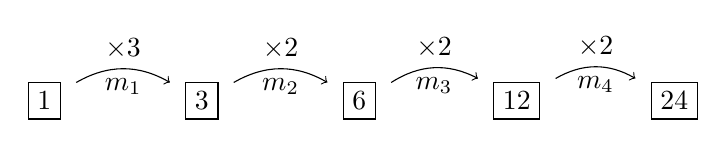
\begin{tikzpicture}
	% \node[draw, rectangle, outer sep=2mm] (n1) at (0,0) {1};
	% \node[draw, rectangle, outer sep=2mm] (n2) at (2,0) {3};
	% \node[draw, rectangle, outer sep=2mm] (n3) at (4,0) {6};
	% \node[outer sep=2mm] (n4) at (6,0) {\ldots};
	% \node[draw, rectangle, outer sep=2mm] (n5) at (8,0) {x};

	% \draw[->, bend left] (n1) tonode[midway,below] {$m_1$} node[midway,above] {$\times 3$} (n2);
	% \draw[->, bend left] (n2) tonode[midway,below] {$m_2$} node[midway,above] {$\times 2$} (n3);
	% \draw[->, bend left] (n3) tonode[midway,below] {$m_3$}  (n4);
	% \draw[->, bend left] (n4) tonode[midway,below] {$m_{n-1}$}  (n5);
	
	\node[draw, rectangle, outer sep=2mm] (n1) at (0,0) {1};
	\node[draw, rectangle, outer sep=2mm] (n2) at (2,0) {3};
	\node[draw, rectangle, outer sep=2mm] (n3) at (4,0) {6};
	\node[draw, rectangle, outer sep=2mm] (n4) at (6,0) {12};
	\node[draw, rectangle, outer sep=2mm] (n5) at (8,0) {24};

	\draw[->, bend left] (n1) to node[midway,below] {$m_1$} node[midway,above] {$\times 3$} (n2);
	\draw[->, bend left] (n2) to node[midway,below] {$m_2$} node[midway,above] {$\times 2$} (n3);
	\draw[->, bend left] (n3) to node[midway,below] {$m_3$} node[midway,above] {$\times 2$} (n4);
	\draw[->, bend left] (n4) to node[midway,below] {$m_4$} node[midway,above] {$\times 2$} (n5);
\end{tikzpicture}
		}
		\caption{Generation of a small example series of periods by multiplication}
	\end{subfigure}
	\hfill
	\begin{subfigure}[c]{0.45\textwidth}
		\resizebox{\textwidth}{!}{%
			\label{fig:chain_of_tasks}
			% \usetikzlibrary{patterns} % Load patterns library
\begin{tikzpicture}
	% \node[draw, rectangle, outer sep=2mm] (n1) at (0,0) {1};
	% \node[draw, rectangle, outer sep=2mm] (n2) at (2,0) {3};
	% \node[draw, rectangle, outer sep=2mm] (n3) at (4,0) {6};
	% \node[outer sep=2mm] (n4) at (6,0) {\ldots};
	% \node[draw, rectangle, outer sep=2mm] (n5) at (8,0) {x};

	% \draw[->, bend left] (n1) tonode[midway,below] {$m_1$} node[midway,above] {$\times 3$} (n2);
	% \draw[->, bend left] (n2) tonode[midway,below] {$m_2$} node[midway,above] {$\times 2$} (n3);
	% \draw[->, bend left] (n3) tonode[midway,below] {$m_3$}  (n4);
	% \draw[->, bend left] (n4) tonode[midway,below] {$m_{n-1}$}  (n5);
	
	\node[draw, rectangle, outer sep=2mm] (n1) at (0,0) {$P=1$};
	\node[draw, rectangle, outer sep=2mm] (n2) at (2,0) {$P=3$};
	\node[draw, rectangle, outer sep=2mm] (n3) at (4,0) {$P=6$};
	\node[draw, rectangle, outer sep=2mm] (n4) at (6,0) {$P=12$};
	\node[draw, rectangle, outer sep=2mm] (n5) at (8,0) {$P=24$};

	\node[draw, rectangle, outer sep=2mm] (n1) at (-1.5,-1) {chain 1};
	\node[draw, rectangle, outer sep=2mm] (n2) at (-1.5,-2) {chain 2};
	\node[draw, rectangle, outer sep=2mm] (n3) at (-1.5,-3) {chain 3};

	\draw[thick, fill=black!60, pattern=none] plot[] coordinates { (-0.5 + 0, -0.5)	(0.5 + 0, -0.5)	(0.5 + 0, -3.5)	(-0.5 + 0,-3.5)	} -- cycle;
	\draw[thick, fill=black!60, pattern=none] plot[] coordinates { (-0.5 + 2, -0.5)	(0.5 + 2, -0.5)	(0.5 + 2, -3.5)	(-0.5 + 2,-3.5)	} -- cycle;
	\draw[thick, fill=black!60, pattern=none] plot[] coordinates { (-0.5 + 4, -0.5)	(0.5 + 4, -0.5)	(0.5 + 4, -3.5)	(-0.5 + 4,-3.5)	} -- cycle;
	\draw[thick, fill=black!60, pattern=none] plot[] coordinates { (-0.5 + 6, -0.5)	(0.5 + 6, -0.5)	(0.5 + 6, -3.5)	(-0.5 + 6,-3.5)	} -- cycle;
	\draw[thick, fill=black!60, pattern=none] plot[] coordinates { (-0.5 + 8, -0.5)	(0.5 + 8, -0.5)	(0.5 + 8, -3.5)	(-0.5 + 8,-3.5)	} -- cycle;

	% chain 1
	\node[draw, rectangle, outer sep=1mm] (T1) at (0,-1) {$\Tau_1$};
	\node[draw, rectangle, outer sep=1mm] (T2) at (2,-1) {$\Tau_2$};
	\node[draw, rectangle, outer sep=1mm] (T3) at (4,-1) {$\Tau_3$};
	\node[draw, rectangle, outer sep=1mm] (T4) at (6,-1) {$\Tau_4$};
	\node[draw, rectangle, outer sep=1mm] (T5) at (8,-1) {$\Tau_5$};
	
	% chain 2
	\node[draw, rectangle, outer sep=1mm] (T6) at (0,-2) {$\Tau_6$};
	\node[draw, rectangle, outer sep=1mm] (T7) at (2,-2) {$\Tau_7$};
	% 												
	\node[draw, rectangle, outer sep=1mm] (T8) at (6,-2) {$\Tau_8$};
	% 											
	
	% chain 3
	\node[draw, rectangle, outer sep=1mm] (T9) at (0,-3) {$\Tau_9$};
	\node[draw, rectangle, outer sep=1mm] (T10) at (2,-3) {$\Tau_{10}$};
	\node[draw, rectangle, outer sep=1mm] (T11) at (4,-3) {$\Tau_{11}$};
	%
	%
  

\draw[->] (T1) to (T2);
\draw[->] (T2) to (T3);
\draw[->] (T3) to (T4);
\draw[->] (T4) to (T5);
\draw[->] (T6) to (T7);
\draw[->] (T7) to (T8);
\draw[->] (T9) to (T10);
\draw[->] (T10) to (T11);

% \draw[->, bend left] (n1) to node[midway,below] {$m_1$} node[midway,above] {$\times 3$} (n2);

		

\end{tikzpicture}
		}
		\caption{Task-set $\Tau=\{\Tau_{1}, \ldots, \Tau_{11}\}$ parted into three subsets each a representation of a chain of inter-task communication}
	\end{subfigure}
	\begin{subfigure}[c]{0.450\textwidth}
		\resizebox{\textwidth}{!}{%
			\label{fig:graph_of_periods}
			% \usetikzlibrary{patterns} % Load patterns library
\begin{tikzpicture}
	\node[draw, circle, inner sep=1mm] (L1-00) at (23 , 8) {$P2_-00$};

	\node[draw, circle, inner sep=1mm] (L2-00) at (11 , 6) {$P1_-00$};
	\node[draw, circle, inner sep=1mm] (L2-01) at (35 , 6) {$P1_-01$};

	\node[draw, circle, inner sep=1mm] (L3-00) at ( 5 , 4) {$P6_00$};
	\node[draw, circle, inner sep=1mm] (L3-01) at (17 , 4) {$P6_01$};
	\node[draw, circle, inner sep=1mm] (L3-02) at (29 , 4) {$P6_02$};
	\node[draw, circle, inner sep=1mm] (L3-03) at (41 , 4) {$P6_03$};

	\node[draw, circle, inner sep=1mm] (L4-00) at ( 2 , 2) {$P3_00$};
	\node[draw, circle, inner sep=1mm] (L4-01) at ( 8 , 2) {$P3_01$};
	\node[draw, circle, inner sep=1mm] (L4-02) at (14 , 2) {$P3_02$};
	\node[draw, circle, inner sep=1mm] (L4-03) at (20 , 2) {$P3_03$};
	\node[draw, circle, inner sep=1mm] (L4-04) at (26 , 2) {$P3_04$};
	\node[draw, circle, inner sep=1mm] (L4-05) at (32 , 2) {$P3_05$};
	\node[draw, circle, inner sep=1mm] (L4-06) at (38 , 2) {$P3_06$};
	\node[draw, circle, inner sep=1mm] (L4-07) at (44 , 2) {$P3_07$};

	\node[draw, circle, inner sep=1mm] (L5-00) at ( 0 , 0) {$P1_00$};
	\node[draw, circle, inner sep=1mm] (L5-01) at ( 2 , 0) {$P1_01$};
	\node[draw, circle, inner sep=1mm] (L5-02) at ( 4 , 0) {$P1_02$};
	\node[draw, circle, inner sep=1mm] (L5-03) at ( 6 , 0) {$P1_03$};
	\node[draw, circle, inner sep=1mm] (L5-04) at ( 8 , 0) {$P1_04$};
	\node[draw, circle, inner sep=1mm] (L5-05) at (10 , 0) {$P1_05$};
	\node[draw, circle, inner sep=1mm] (L5-06) at (12 , 0) {$P1_06$};
	\node[draw, circle, inner sep=1mm] (L5-07) at (14 , 0) {$P1_07$};
	\node[draw, circle, inner sep=1mm] (L5-08) at (16 , 0) {$P1_08$};
	\node[draw, circle, inner sep=1mm] (L5-09) at (18 , 0) {$P1_09$};
	\node[draw, circle, inner sep=1mm] (L5-10) at (20 , 0) {$P1_10$};
	\node[draw, circle, inner sep=1mm] (L5-11) at (22 , 0) {$P1_11$};
	\node[draw, circle, inner sep=1mm] (L5-12) at (24 , 0) {$P1_12$};
	\node[draw, circle, inner sep=1mm] (L5-13) at (26 , 0) {$P1_13$};
	\node[draw, circle, inner sep=1mm] (L5-14) at (28 , 0) {$P1_14$};
	\node[draw, circle, inner sep=1mm] (L5-15) at (30 , 0) {$P1_15$};
	\node[draw, circle, inner sep=1mm] (L5-16) at (32 , 0) {$P1_16$};
	\node[draw, circle, inner sep=1mm] (L5-17) at (34 , 0) {$P1_17$};
	\node[draw, circle, inner sep=1mm] (L5-18) at (36 , 0) {$P1_18$};
	\node[draw, circle, inner sep=1mm] (L5-19) at (38 , 0) {$P1_19$};
	\node[draw, circle, inner sep=1mm] (L5-20) at (40 , 0) {$P1_20$};
	\node[draw, circle, inner sep=1mm] (L5-21) at (42 , 0) {$P1_21$};
	\node[draw, circle, inner sep=1mm] (L5-22) at (44 , 0) {$P1_22$};
	\node[draw, circle, inner sep=1mm] (L5-23) at (46 , 0) {$P1_23$};

	\draw[->] (L1-00) to (L2-00);
	\draw[->] (L1-00) to (L2-01);

	\draw[->] (L2-00) to (L3-00);
	\draw[->] (L2-00) to (L3-01);
	\draw[->] (L2-01) to (L3-02);
	\draw[->] (L2-01) to (L3-03);

	\draw[->] (L3-00) to (L4-00);
	\draw[->] (L3-00) to (L4-01);
	\draw[->] (L3-01) to (L4-02);
	\draw[->] (L3-01) to (L4-03);
	\draw[->] (L3-02) to (L4-04);
	\draw[->] (L3-02) to (L4-05);
	\draw[->] (L3-03) to (L4-06);
	\draw[->] (L3-03) to (L4-07);

	\draw[->] (L4-00) to (L5-00);
	\draw[->] (L4-00) to (L5-01);
	\draw[->] (L4-00) to (L5-02);
	\draw[->] (L4-01) to (L5-03);
	\draw[->] (L4-01) to (L5-04);
	\draw[->] (L4-01) to (L5-05);
	\draw[->] (L4-02) to (L5-06);
	\draw[->] (L4-02) to (L5-07);
	\draw[->] (L4-02) to (L5-08);
	\draw[->] (L4-03) to (L5-09);
	\draw[->] (L4-03) to (L5-10);
	\draw[->] (L4-03) to (L5-11);
	\draw[->] (L4-04) to (L5-12);
	\draw[->] (L4-04) to (L5-13);
	\draw[->] (L4-04) to (L5-14);
	\draw[->] (L4-05) to (L5-15);
	\draw[->] (L4-05) to (L5-16);
	\draw[->] (L4-05) to (L5-17);
	\draw[->] (L4-06) to (L5-18);
	\draw[->] (L4-06) to (L5-19);
	\draw[->] (L4-06) to (L5-20);
	\draw[->] (L4-07) to (L5-21);
	\draw[->] (L4-07) to (L5-22);
	\draw[->] (L4-07) to (L5-23);

	\draw[line width=2mm, loosely dotted, pattern=none] plot[] coordinates { (-1, -1) (11, -1) (11, 5) (-1, 5) } -- cycle;
\end{tikzpicture}
		}
		\caption{A graph depicting the generated periods. Highlighted with a dotted box: subtree with $P6_0$ as root (see \cref{fid:graph_of_tasks}).}
	\end{subfigure}
	\hfill
	\begin{subfigure}[c]{0.45\textwidth}
		\resizebox{\textwidth}{!}{%
			\label{fig:graph_of_tasks}
			% \usetikzlibrary{patterns} % Load patterns library
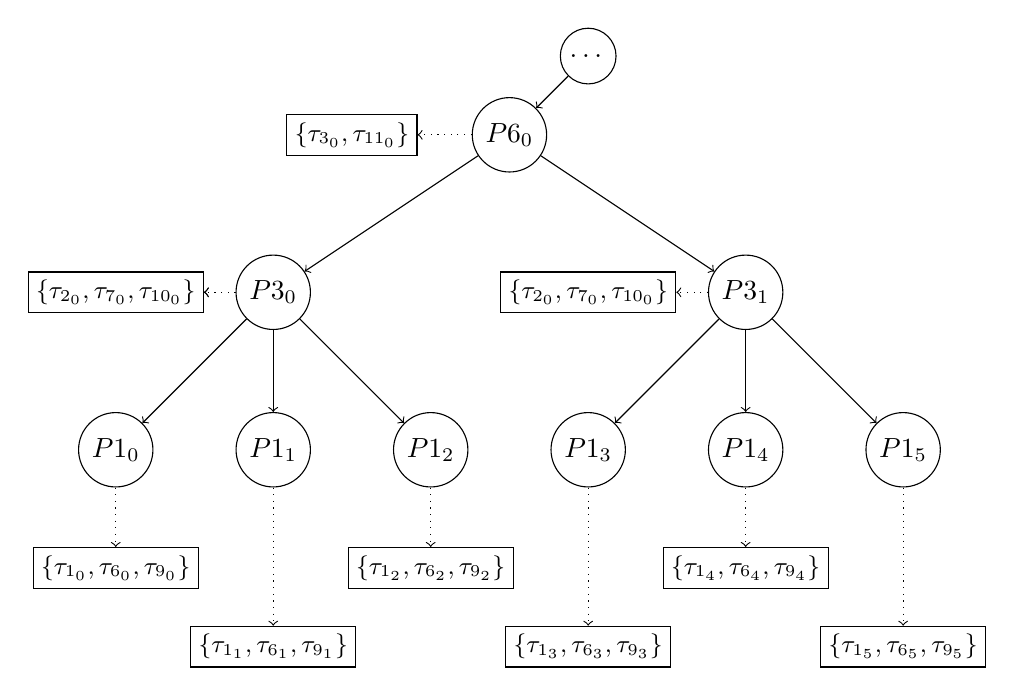
\begin{tikzpicture}
	\node[draw, circle, inner sep=1mm] (L2-00) at ( 6, 5) {\ldots};

	\node[draw, circle, inner sep=1mm] (L3-00) at ( 5 , 4) {$P6_0$};

	\node[draw, circle, inner sep=1mm] (L4-00) at ( 2 , 2) {$P3_0$};
	\node[draw, circle, inner sep=1mm] (L4-01) at ( 8 , 2) {$P3_1$};

	\node[draw, circle, inner sep=1mm] (L5-00) at ( 0 , 0) {$P1_0$};
	\node[draw, circle, inner sep=1mm] (L5-01) at ( 2 , 0) {$P1_1$};
	\node[draw, circle, inner sep=1mm] (L5-02) at ( 4 , 0) {$P1_2$};
	\node[draw, circle, inner sep=1mm] (L5-03) at ( 6 , 0) {$P1_3$};
	\node[draw, circle, inner sep=1mm] (L5-04) at ( 8 , 0) {$P1_4$};
	\node[draw, circle, inner sep=1mm] (L5-05) at (10 , 0) {$P1_5$};

	\node[draw, rectangle, inner sep=1mm, align=center] (L3-T00) at ( 3 , 4) {\small $\{\tau_{3_0},\tau_{11_0}\}$};

	\node[draw, rectangle, inner sep=1mm, align=center] (L4-T00) at ( 0 , 2) {\small $\{\tau_{2_0},\tau_{7_0},\tau_{10_0}\}$};
	\node[draw, rectangle, inner sep=1mm, align=center] (L4-T01) at ( 6 , 2) {\small $\{\tau_{2_0},\tau_{7_0},\tau_{10_0}\}$};

	\node[draw, rectangle, inner sep=1mm, align=center] (L5-T00) at ( 0 , -1.5) {\small $\{\tau_{1_0},\tau_{6_0},\tau_{9_0}\}$};
	\node[draw, rectangle, inner sep=1mm, align=center] (L5-T01) at ( 2 , -2.5) {\small $\{\tau_{1_1},\tau_{6_1},\tau_{9_1}\}$};
	\node[draw, rectangle, inner sep=1mm, align=center] (L5-T02) at ( 4 , -1.5) {\small $\{\tau_{1_2},\tau_{6_2},\tau_{9_2}\}$};
	\node[draw, rectangle, inner sep=1mm, align=center] (L5-T03) at ( 6 , -2.5) {\small $\{\tau_{1_3},\tau_{6_3},\tau_{9_3}\}$};
	\node[draw, rectangle, inner sep=1mm, align=center] (L5-T04) at ( 8 , -1.5) {\small $\{\tau_{1_4},\tau_{6_4},\tau_{9_4}\}$};
	\node[draw, rectangle, inner sep=1mm, align=center] (L5-T05) at (10 , -2.5) {\small $\{\tau_{1_5},\tau_{6_5},\tau_{9_5}\}$};

	\draw[->] (L2-00) to (L3-00);

	\draw[->] (L3-00) to (L4-00);
	\draw[->] (L3-00) to (L4-01);

	\draw[->] (L4-00) to (L5-00);
	\draw[->] (L4-00) to (L5-01);
	\draw[->] (L4-00) to (L5-02);
	\draw[->] (L4-01) to (L5-03);
	\draw[->] (L4-01) to (L5-04);
	\draw[->] (L4-01) to (L5-05);

	\draw[->,dotted] (L3-00) to (L3-T00);
	\draw[->,dotted] (L4-00) to (L4-T00);
	\draw[->,dotted] (L4-00) to (L4-T00);
	\draw[->,dotted] (L4-01) to (L4-T01);
	\draw[->,dotted] (L5-00) to (L5-T00);
	\draw[->,dotted] (L5-01) to (L5-T01);
	\draw[->,dotted] (L5-02) to (L5-T02);
	\draw[->,dotted] (L5-03) to (L5-T03);
	\draw[->,dotted] (L5-04) to (L5-T04);
	\draw[->,dotted] (L5-05) to (L5-T05);

\end{tikzpicture}
		}
		\caption{Subgraph of \cref{fig:graph_of_periods} showing the jobs associated to each representation of period iteration}
	\end{subfigure}
	\caption{Generation of periods and task-set with tasks with given period}
\end{figure}

\subsection{Generating Task Chains}\label{sec:generating_task_chains}
To generate the task-set multiple tasks will be iteratively added and assigned to the already generated periods.
By iterating about given period values a natural order of the tasks' periods is assured.
With choosing the \ac{RMS} as scheduling method it is an descending order of priority, since the higher periods will result in lower priorities.
Knowing this the tasks can be connected with its successor (if one does exist) to limit the inter-task communication to be directed from higher priorities to lower priorities.
Doing so the sender is assured to run earlier in respect to the receiver, if no locking or priority inversion is apparent. \todo{priority inversion and resource locking in model}
By skipping a period while generating the tasks, the chains are built to vary the length and distribution of their associated tasks.
The skip may be done at random. \todo{explain random as random with seed}

\subsection{Creating Conditions}\label{sec:creating_conditions}
\todo{conditions}

\subsection{Spreading Server Model into Instances}\label{sec:spreading_server_model_into_instances}
By using a harmonic task-set it is possible to fan out the given list of periods as seen in \cref{fig:chain_of_periods} into a tree structure as seen in \cref{fig:graph_of_periods}.
Due to the periods being multiples of each other, the used multiple is the key to perfectly map the periods onto the same span of time.
Beginning with the smallest period i.e. $1$, whilst ignoring the periods greater than that for now, it is a perfect representation of needed planning cycle $1$.
This is represented by node $P1_0$ in \cref{fig:graph_of_periods}.
If the next biggest period $3$ gets added into the picture, the planning cycle increases to $3$, resulting in three repetitions of previous period to match the newer and bigger cycle, represented by $P3_0$ and $P1_0$ to $P1_2$ in \cref{fig:graph_of_periods}.
Repeating this for the remaining periods, the complete tree, built so far, will be multiplied and added.
The benefits of this design will be explained in more detail in \cref{sec:concept_scheduler}.

\subsection{Assigning Computational Time}\label{sec:concept_load_spread}
At this stage, the generated tasks have no computational time assigned.
The model is planned to satisfy a given utilization.
Taking that utilization, each period may be assigned a combined execution time to represent the sum of associated tasks.

The planning cycle's time frame, multiplied by the predefined utilization, determines the total amount of execution time that can be distributed across the tasks.
This means that for each layer of period nodes in the tree structure, the sum of the execution times of all tasks must not exceed the product of the planning cycle's time frame and the predefined utilization.

For example, if the planning cycle's time frame is 24 units and the predefined utilization is 0.75, the total execution time available for all tasks in that planning cycle is \(24 \times 0.75 = 18\) units.
This 18 units of execution time must be spread across all tasks in the tree, ensuring that the sum of the execution times of tasks associated with each period node does not exceed this limit.

The total execution time for each period layer is then distributed among the tasks assigned to that period. This is done by randomly assigning execution times to each task such that the sum of the execution times equals the total execution time for the period layer.

For example, if a period layer of $P1$ has a total execution time of 6 units and there are 3 tasks $T_1$, $T_3$ and $T_9$ assigned to that period, the execution times could be randomly assigned as $CP_{1_1} = 1$, $CP_{3_1} = 2$, and $CP_{9_1} = 3$, ensuring that the sum is \( CP_{1_1} + $CP_{3_1} + $CP_{9_1} = 6 \) units.

By randomly distributing the execution times in this manner, the system ensures that the overall utilization remains within the desired bounds, maintaining the schedulability and efficiency of the task set.
\todo{check utilization use}
\todo{make sure the times fit. CT<1/2period}

\subsection{Generating Load with Lower Execution Times}\label{sec:concept_lower_execution_times}
For the system to not only represent all tasks \ac{WCET} a variation of execution times per task need to be created.
Since the generated tasks with full load still have schedulability, the execution time of the tasks may be reduced without compromising the schedulability.
For that reason the execution time of each task is multiplied with a random value between zero and one until a sufficient amount of different values is generated.
Keeping the increasing complexity in mind, the system is designed to use a discrete distribution instead of continuous value functions. \todo{value functions more complex than discrete? source}

\subsection{Building a Scheduler and Performing Schedulability Test}\label{sec:concept_scheduler}
The schedule can be generated by performing a depth-first traversal of the previously described tree structure.
The leaves of the tree represent the tasks with the highest priority and are processed first during the traversal.
As the traversal continues, tasks in higher layers with lower priorities are processed until the root is reached.
Starting with an empty schedule for the given planning cycle the execution times of the highest prioritized tasks can simply be added.
If one layer is added to the schedule, the next layer with the next next higher priority is added to fill the remaining idle time.
Since the time and utilization are previously calculated it is ensured the 

\todo{prio for equal periods -> arbritrary, but predictable order.}

\todo{building a scheduler (schedulability test)}

\subsection{Exporting Task-Set}\label{sec:exporting_task_set}
\todo{exporting task-set}

\section{Implementation}
\label{sec:implementation}


\section{Tasks with Release Times and Execution Times}
\label{sec:tasks_release_execution}

In real-time systems, tasks are characterized by their release times and execution times.
The release time of a task is the time at which the task becomes ready for execution.
Execution times can vary depending on the complexity and requirements of the task.

Consider a set of tasks \( \tau = \{\tau_1, \tau_2, \ldots, \tau_n\} \).
Each task \( \tau_i \) has a release time \( r_i \) and a list of possible execution times \( \{e_{i1}, e_{i2}, \ldots, e_{im}\} \).
The release time \( r_i \) indicates when the task \( \tau_i \) is ready to be executed, and the list of execution times represents the different durations the task might take to complete under various conditions.
The release times will be constrained further in the section \cref{sec:harmonic_task_set}.

For example, let us define three tasks with their respective release times and execution times:

\begin{itemize}
	\item Task \( \tau_1 \): Release time \( r_1 = 0 \), Execution times \( \{3, 4, 5\} \)
	\item Task \( \tau_2 \): Release time \( r_2 = 2 \), Execution times \( \{2, 3\} \)
	\item Task \( \tau_3 \): Release time \( r_3 = 4 \), Execution times \( \{1, 2, 3\} \)
\end{itemize}

The scheduler must consider both the release times and the possible execution times to ensure that all tasks meet their deadlines.
Each task will be assigned a hard deadline which strictly encases the time frame a task may be scheduled in. 
This involves determining the optimal order of execution and allocating sufficient resources to handle the variability in execution times.

By analyzing the release times and execution times, we can develop strategies to improve the efficiency and reliability of real-time systems, ensuring that tasks are completed within their required time frames.

\section{Flow of Data}
\label{sec:flow_of_data}

\section{Creating Conditions}
\label{sec:creating_conditions}

\section{Representation}
\label{sec:representation}